\documentclass[10pt, letterpaper]{report}

%% packages
\usepackage[utf8]{inputenc}
\usepackage[T1]{fontenc}
\usepackage[spanish, mexico]{babel}
\usepackage{titlesec}
\usepackage{glossaries}
\usepackage{graphicx}
\usepackage{array}
\usepackage{multirow}
\usepackage{lscape}

%% page settings
\usepackage[top=2cm, bottom=1.8cm, left=2.5cm, right=2.5cm]{geometry} % for page border settings
\usepackage{fancyhdr} % for head and footer options

%% commands
\newcommand{\tbi}[1]{\textbf{\textit{#1}}}

%% glossary
\makeglossaries
\newglossaryentry{Sucursal}
{
	name={Sucursal},
	description={Sucursal de la Agencia de Renta de Autos.}
}
\newglossaryentry{ModeloAuto}
{
	name={Modelo de Auto},
	description={Modelo del Auto a la renta.}
}

\begin{document}

\title{Requerimientos Funcionales (EU-Car)}
\author{Softtek}
\date{}
\maketitle

\pagestyle{plain}
\tableofcontents

\chapter{Modelo de Dominio}

%\section{Diagrama} \label{sec:uml-domain-model}

\begin{figure}[h]
	\label{tab:uml-domain-model}
	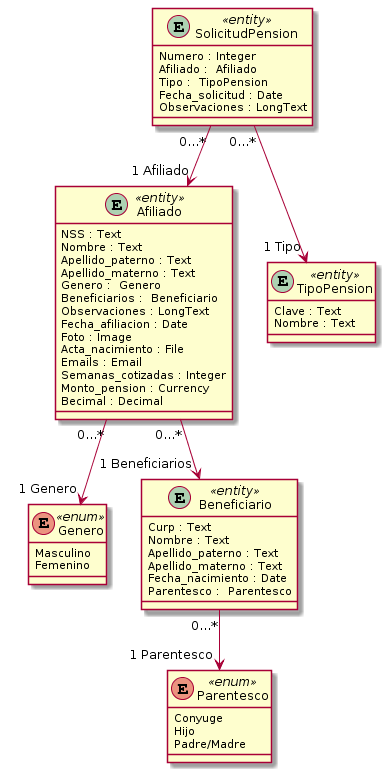
\includegraphics[width=0.5\textwidth]{uml-diagrams/domain-model.png}
	\caption{Modelo de Dominio}
\end{figure}

\section{Descripción de las Entidades de Negocio} \label{sec:entity-description}

\begin{table}[h]
	\caption{Entidades del Modelo de Dominio}
	\label{tab:entities}
	%\resizebox{\textwidth}{!}{
	\begin{center}
	\begin{tabular}{ l l } 
		\hline
		\textbf{Entidad} & \textbf{Descripción} \\
		\hline
		Solicitud Pensión & Información de la Solicitud de Pensión derivada del derecho de un Afiliado al IMSS. \\ 
		\hline
	\end{tabular}
	\end{center}
	%}
\end{table}

\section{Campos por Entidad de Negocio} \label{sec:entity-fields}

\begin{table}[h]
	\caption{Entidad de Negocio: Solicitud Pensión}
	\label{tab:fields-solicitudpension}
	%\resizebox{\textwidth}{!}{
	\begin{center}
	\begin{tabular}{ l l l l } 
		\hline
		\textbf{Campo} & \textbf{Tipo} & \textbf{Restricciones} & \textbf{Descripción} \\
		\hline
		Número & Integer & Required: true & Número de la Solicitud generado automáticamente. \\ 
		\hline
	\end{tabular}
	\end{center}
	%}
\end{table}

\chapter{Casos de Uso}

%\pagestyle{fancy}
%\fancyhf{}
%\fancyhead[OC]{\leftmark}
%\fancyhead[EC]{\rightmark}
%\cfoot{\thepage}

\section{Modulo: Modelo de Autos} \label{sec:cumodeloautoservices}

\subsection{UC05. Crear un Modelo de Auto} \label{sec:cucrearmodeloauto}

\begin{tabular}{ p{3.5cm} p{11.5cm} }
	\textbf{Actores} & Administrador \\
	\textbf{Objetivo} & EU-Rent decide ofrecer a sus Clientes un nuevo modelo de Auto. \\
	\textbf{Evento Disparador} & Administrador solicita la página \textit{[Crear Modelo de Auto]}. \\
	\textbf{Tipo} & Usuario \\
	\\
\end{tabular}

\begin{tabular}{ p{15.5cm} }
	\textbf{Escenario Principal} \\
	\begin{enumerate}
		\item El Sistema muestra la página \textit{[Crear Modelo de Auto]}.
		\item Administrador captura información en la forma \textit{[Crear Modelo de Auto]}.
		\item Administrador elige el comando \textit{[Guardar]}.
		\item El Sistema valida que los datos de la forma \textit{[Crear Modelo de Auto]} estan completos.
			\begin{enumerate}
				\item Excepción: Datos incompletos.
			\end{enumerate}
		\item El Sistema crea un nuevo registro en la entidad \textit{[ModeloAuto]}.
		\item Fin del Caso de Uso.
	\end{enumerate} \\
\end{tabular}




\subsection{UC06. Buscar un Modelo de Auto} \label{sec:cubuscarmodeloauto}
\textbf{Actores}: Administrador

\textbf{Objetivo}: EU-Rent decide buscar un Modelo de Auto para editarlo o eliminarlo.

\textbf{Evento Disparador}: Administrador solicita la página \textit{[Buscar Modelo de Auto]}.

\textbf{Tipo}: Usuario\\

\textbf{Escenario Principal}

\begin{enumerate}
\item El Sistema muestra la página \textit{[Buscar Modelo de Auto]}.
\item Administrador captura información en la forma \textit{[Criterios de Búsqueda]}.
\item Administrador elige el comando \textit{[Buscar]}.
\item El Sistema valida que los datos de la forma \textit{[Criterios de Búsqueda]} estan completos.
	\begin{enumerate}
		\item Excepción: Datos incompletos.
	\end{enumerate}
\item El Sistema obtiene información y muestra la lista \textit{[Resultados de Búsqueda]}.
\item Fin del Caso de Uso.
\end{enumerate}
\subsection{UC07. Editar un Modelo de Auto} \label{sec:cueditarmodeloauto}
\textbf{Actores}: Administrador

\textbf{Objetivo}: EU-Rent decide modificar los datos de un Modelo de Auto.

\textbf{Evento Disparador}: Administrador solicita la página \textit{[Editar Modelo de Auto]}.

\textbf{Tipo}: Usuario\\

\textbf{Escenario Principal}

\begin{enumerate}
\item El Sistema invoca al Caso de Uso \textit{[UC06. Buscar un Modelo de Auto]}.
\item Administrador selecciona el comando \textit{[Editar]}.
\item El Sistema muestra la página \textit{[Editar Modelo de Auto]}.
\item Administrador captura información en la forma \textit{[Editar Modelo de Auto]}.
\item Administrador elige el comando \textit{[Guardar]}.
\item El Sistema valida que los datos de la forma \textit{[Editar Modelo de Auto]} estan completos.
	\begin{enumerate}
		\item Excepción: Datos incompletos.
	\end{enumerate}
\item El Sistema actuliza la información de la entidad \textit{[ModeloAuto]}.
\item Fin del Caso de Uso.
\end{enumerate}
\subsection{UC08. Eliminar Modelo de Auto} \label{EliminarModeloAuto}
\textbf{Actores}: Administrador

\textbf{Objetivo}: EU Rent decide eliminar un Modelo de Auto existente.

\textbf{Evento Disparador}: Administrador solicita la página \textit{[Eliminar Modelo de Auto]}.

\textbf{Tipo}: Usuario\\

\textbf{Escenario Principal}

\begin{enumerate}
\item El Sistema invoca al Caso de Uso \textit{[UC06. Buscar un Modelo de Auto]}.
\item Administrador selecciona el comando \textit{[Eliminar]}.
\item El Sistema muestra la página \textit{[Eliminar Modelo de Auto]}.
\item Administrador elige el comando \textit{[Eliminar]}.
\item El Sistema elimina el registro de la entidad \textit{[ModeloAuto]}.
\item Fin del Caso de Uso.
\end{enumerate}
\section{Modulo: Sucursales}

\subsection{UC01. Crear una Sucursal} \label{CrearSucursal}
\textbf{Actores}: Administrador

\textbf{Objetivo}: EU-Rent decide abrir una nueva Sucursal.

\textbf{Evento Disparador}: Administrador solicita la página \textit{[Crear Sucursal]}.

\textbf{Tipo}: Usuario\\

\textbf{Escenario Principal}

\begin{enumerate}
\item El Sistema muestra la página \textit{[Crear Sucursal]}.
\item Administrador captura información en la forma \textit{[Crear Sucursal]}.
\item Administrador elige el comando \textit{[Guardar]}.
\item El Sistema valida que los datos de la forma \textit{[Crear Sucursal]} estan completos.
	\begin{enumerate}
		\item Excepción: Datos incompletos.
	\end{enumerate}
\item El Sistema crea un nuevo registro en la entidad \textit{[Sucursal]}.
\item Fin del Caso de Uso.
\end{enumerate}
\subsection{UC02. Buscar una Sucursal} \label{BuscarSucursal}
\textbf{Actores}: Administrador

\textbf{Objetivo}: EU-Rent decide buscar una Sucursal para editarla o eliminarla.

\textbf{Evento Disparador}: Administrador solicita la página \textit{[Buscar Sucursal]}.

\textbf{Tipo}: Usuario\\

\textbf{Escenario Principal}

\begin{enumerate}
\item El Sistema muestra la página \textit{[Buscar Sucursal]}.
\item Administrador captura información en la forma \textit{[Criterios de Búsqueda]}.
\item Administrador elige el comando \textit{[Buscar]}.
\item El Sistema valida que los datos de la forma \textit{[Criterios de Búsqueda]} estan completos.
	\begin{enumerate}
		\item Excepción: Datos incompletos.
	\end{enumerate}
\item El Sistema obtiene información y muestra la lista \textit{[Resultados de Búsqueda]}.
\item Fin del Caso de Uso.
\end{enumerate}
\subsection{UC03. Editar una Sucursal} \label{EditarSucursal}
\textbf{Actores}: Administrador

\textbf{Objetivo}: EU-Rent decide modificar los datos de una Sucursal.

\textbf{Evento Disparador}: Administrador solicita la página \textit{[Editar Sucursal]}.

\textbf{Tipo}: Usuario\\

\textbf{Escenario Principal}

\begin{enumerate}
\item El Sistema invoca al Caso de Uso \textit{[UC02. Buscar una Sucursal]}.
\item Administrador selecciona el comando \textit{[Editar]}.
\item El Sistema muestra la página \textit{[Editar Sucursal]}.
\item Administrador captura información en la forma \textit{[Editar Sucursal]}.
\item Administrador elige el comando \textit{[Guardar]}.
\item El Sistema valida que los datos de la forma \textit{[Editar Sucursal]} estan completos.
	\begin{enumerate}
		\item Excepción: Datos incompletos.
	\end{enumerate}
\item El Sistema actuliza la información de la entidad \textit{[Sucursal]}.
\item Fin del Caso de Uso.
\end{enumerate}
\subsection{UC04. Eliminar Sucursal} \label{EliminarSucursal}
\textbf{Actores}: Administrador

\textbf{Objetivo}: EU Rent decide eliminar una Sucursal existente.

\textbf{Evento Disparador}: Administrador solicita la página \textit{[Eliminar Sucursal]}.

\textbf{Tipo}: Usuario\\

\textbf{Escenario Principal}

\begin{enumerate}
\item El Sistema invoca al Caso de Uso \textit{[UC02. Buscar una Sucursal]}.
\item Administrador selecciona el comando \textit{[Eliminar]}.
\item El Sistema muestra la página \textit{[Eliminar Sucursal]}.
\item Administrador elige el comando \textit{[Eliminar]}.
\item El Sistema elimina el registro de la entidad \textit{[Sucursal]}.
\item Fin del Caso de Uso.
\end{enumerate}


\chapter{Especificación de la Interfaz Gráfica}

\section{Modulo: Sucursales}

\subsection{Crear Sucursal}
\textbf{Descripción}: Permite registrar nuevas Sucursales.\\
\begin{figure}[h]
	\label{tab:layout-crearsucursalpage}
	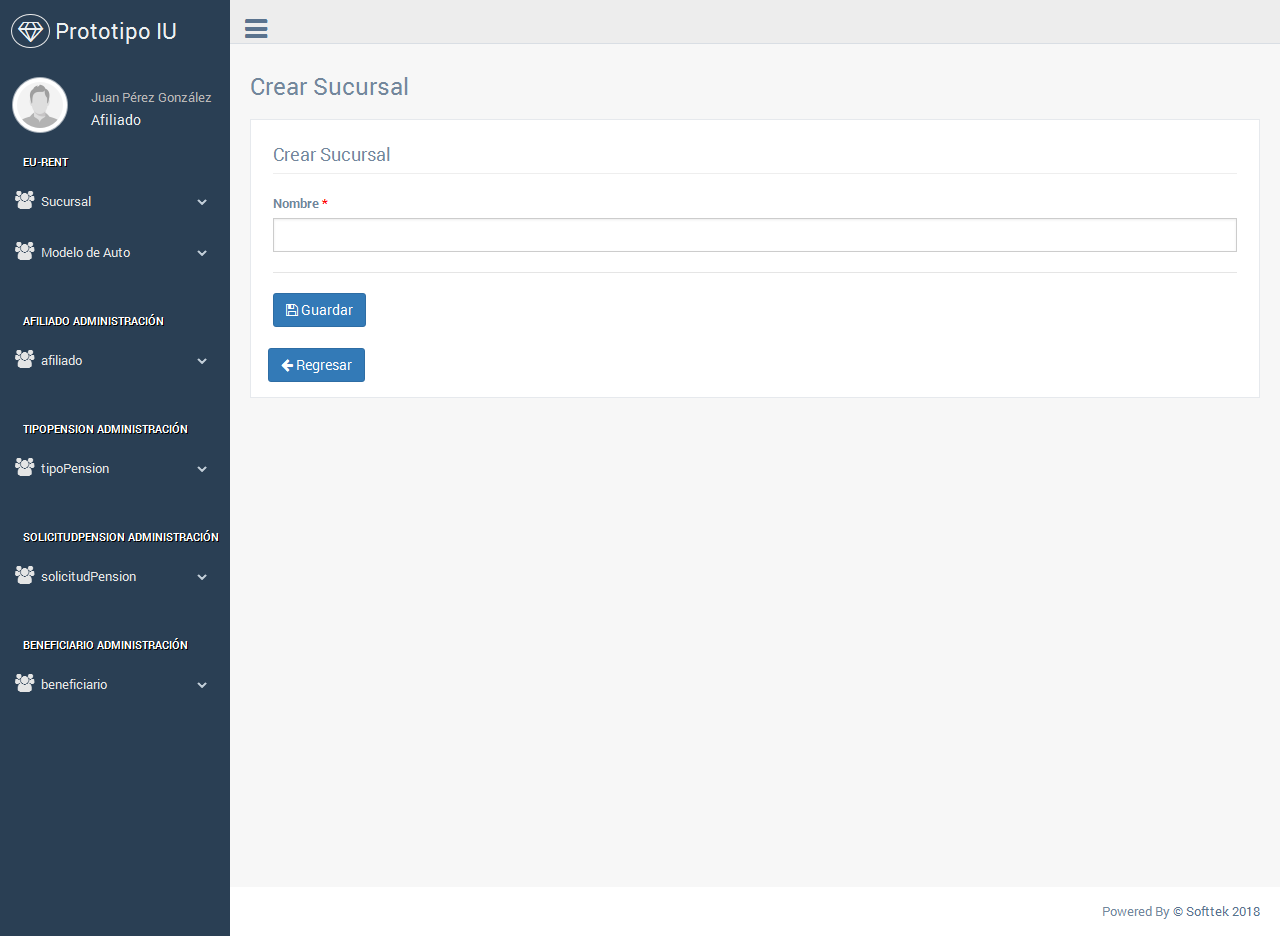
\includegraphics[width=\linewidth]{ui-prototype/SucursalServices/CrearSucursalPage.png}
	\caption{Layout: Crear Sucursal}
\end{figure}

%\begin{landscape}
\begin{table}[t]
	\caption{Forma: Crear Sucursal}
	\label{tab:campos-crearsucursalpage}
	\resizebox{\textwidth}{!}{
	\begin{tabular}{ p{2cm} p{2cm} p{2cm} p{2cm} p{2cm} p{1.5cm} p{3cm} p{4cm} } 
		\hline
		\textbf{Etiqueta} & \textbf{Widget} & \textbf{Default} & \textbf{Tipo} & \textbf{¿Requerido?} & \textbf{E/S} & \textbf{Fuente de Datos} & \textbf{Comentarios} \\
		\hline
		NSS & Texto & Vacío & A(10) & Si & E & Afiliado.Nss & ... \\ 
		\hline
	\end{tabular}
	}
\end{table}
%\end{landscape}


\subsection{Buscar Sucursal}

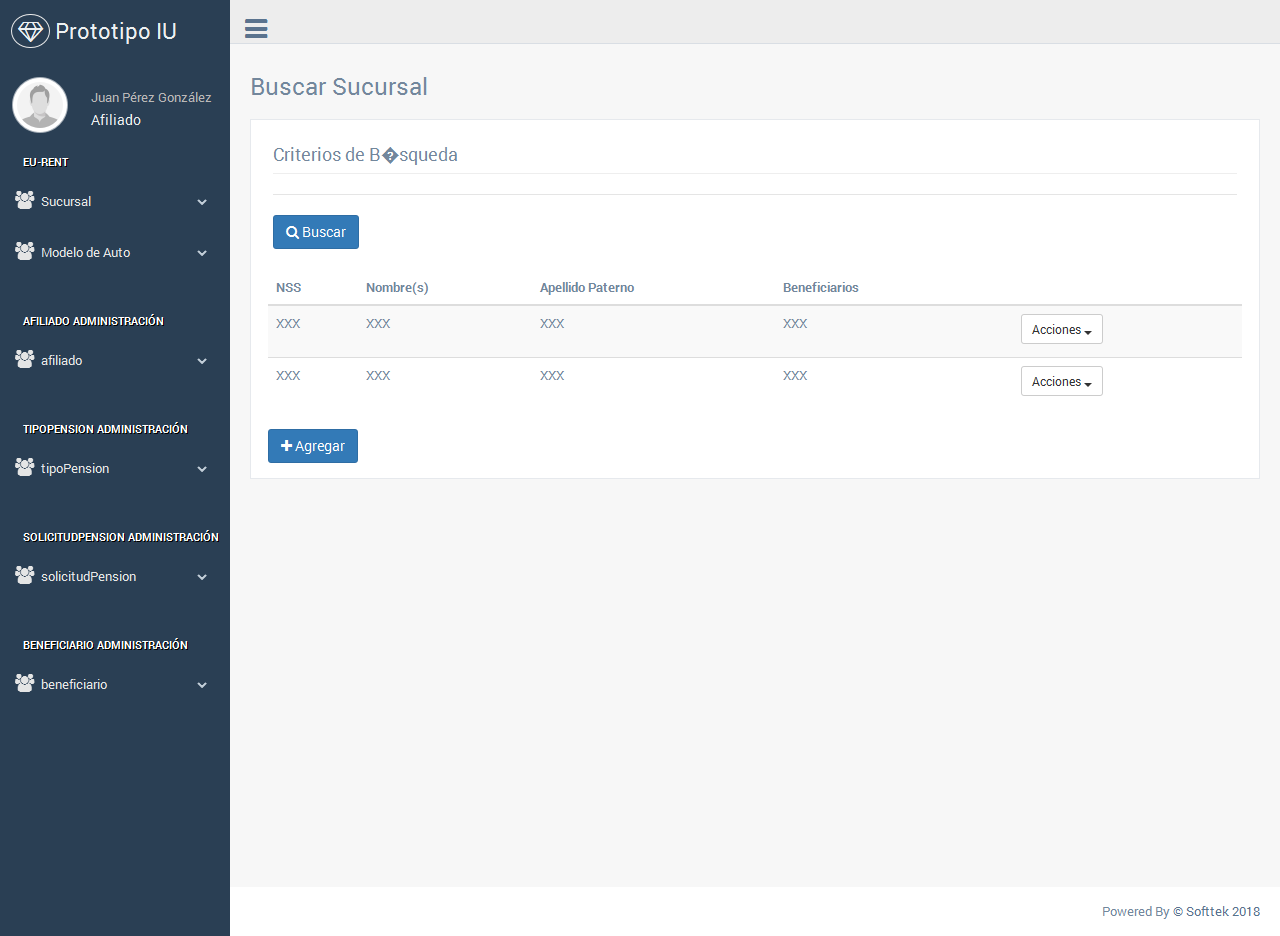
\includegraphics[width=\linewidth]{ui-prototype/SucursalServices/BuscarSucursalPage.png}

\subsection{Editar Sucursal}

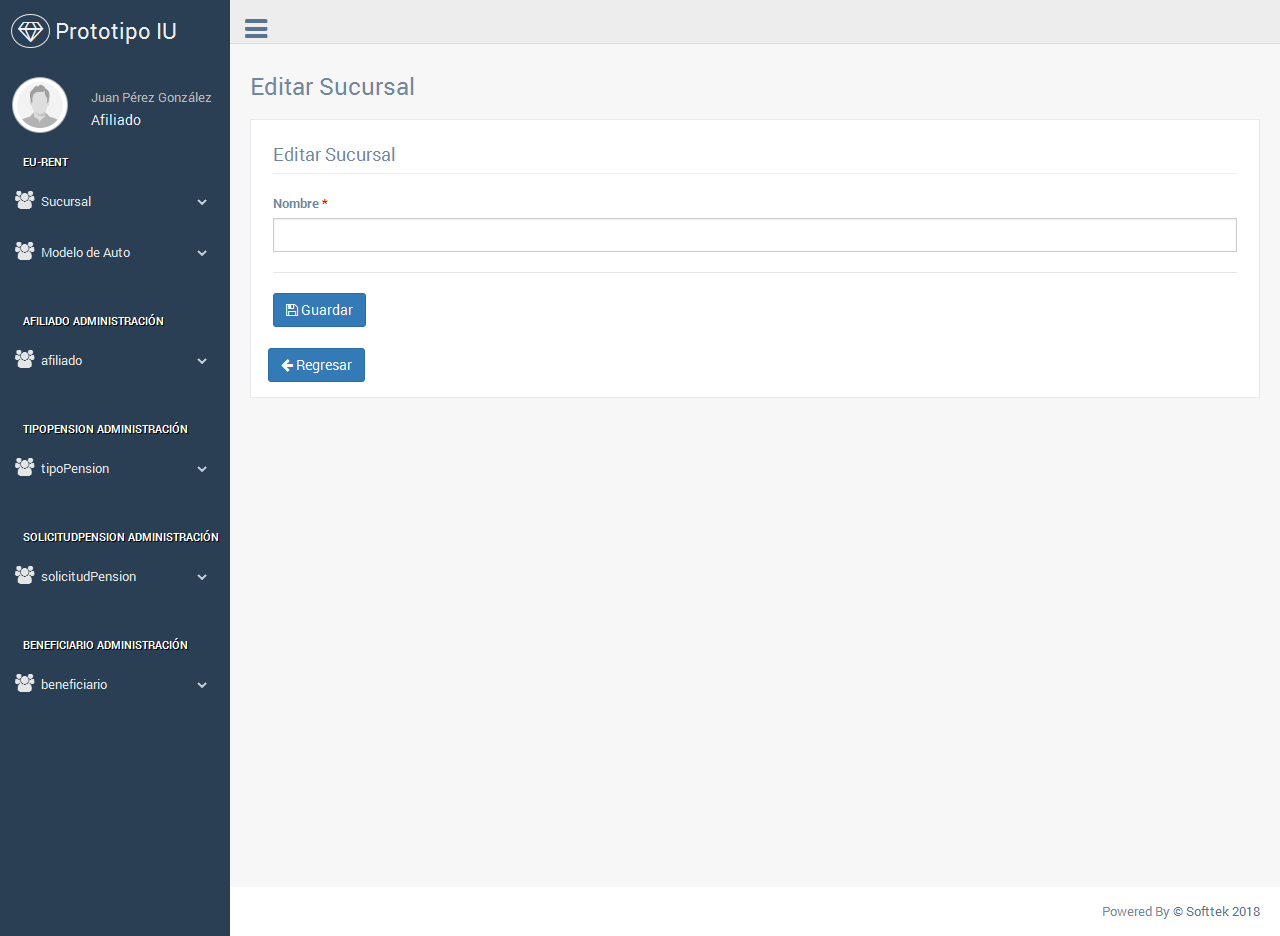
\includegraphics[width=\linewidth]{ui-prototype/SucursalServices/EditarSucursalPage.png}

\subsection{Eliminar Sucursal}

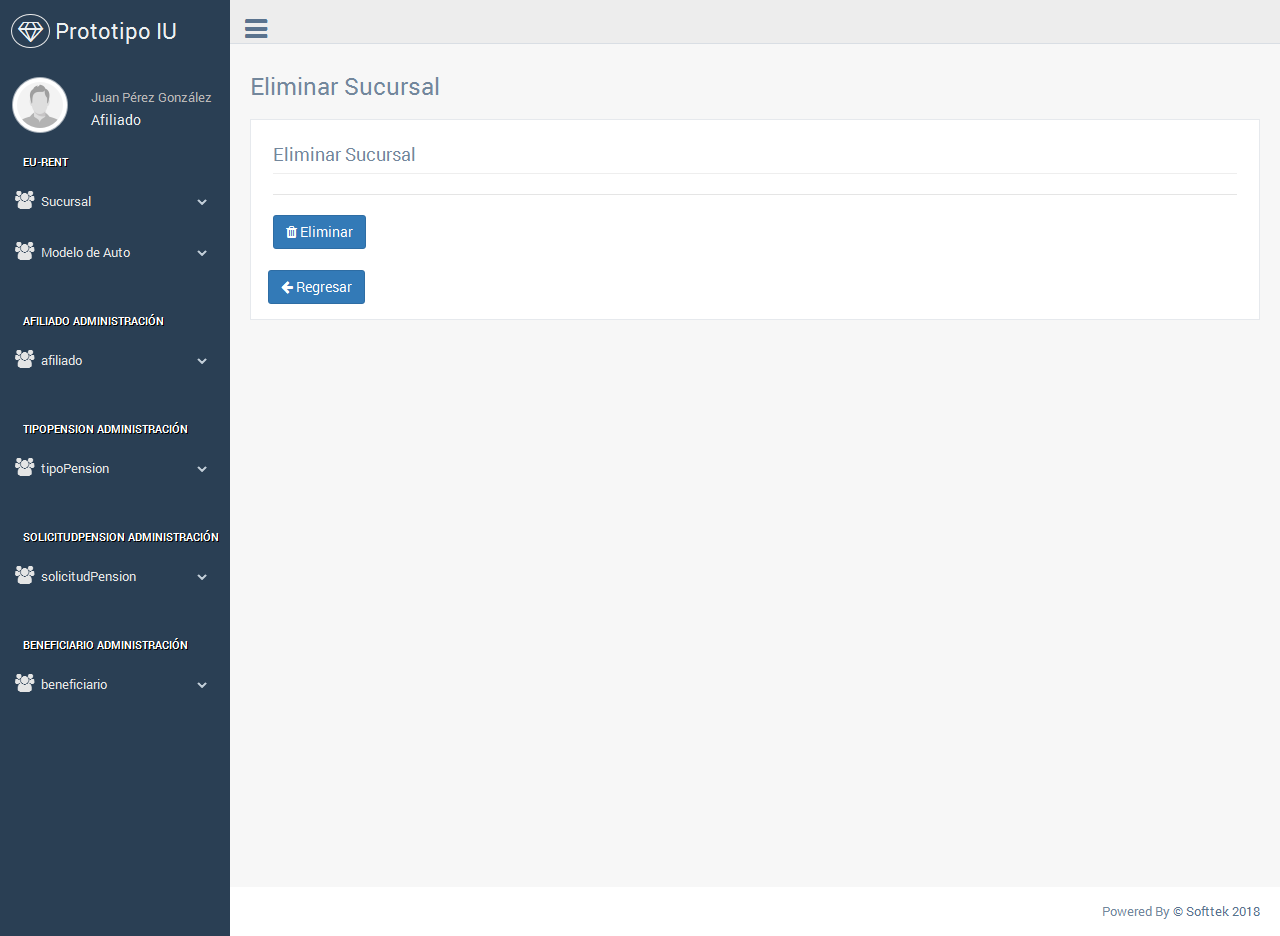
\includegraphics[width=\linewidth]{ui-prototype/SucursalServices/EliminarSucursalPage.png}


\section{Modulo: Modelo de Autos}

\subsection{Crear Modelo de Auto}

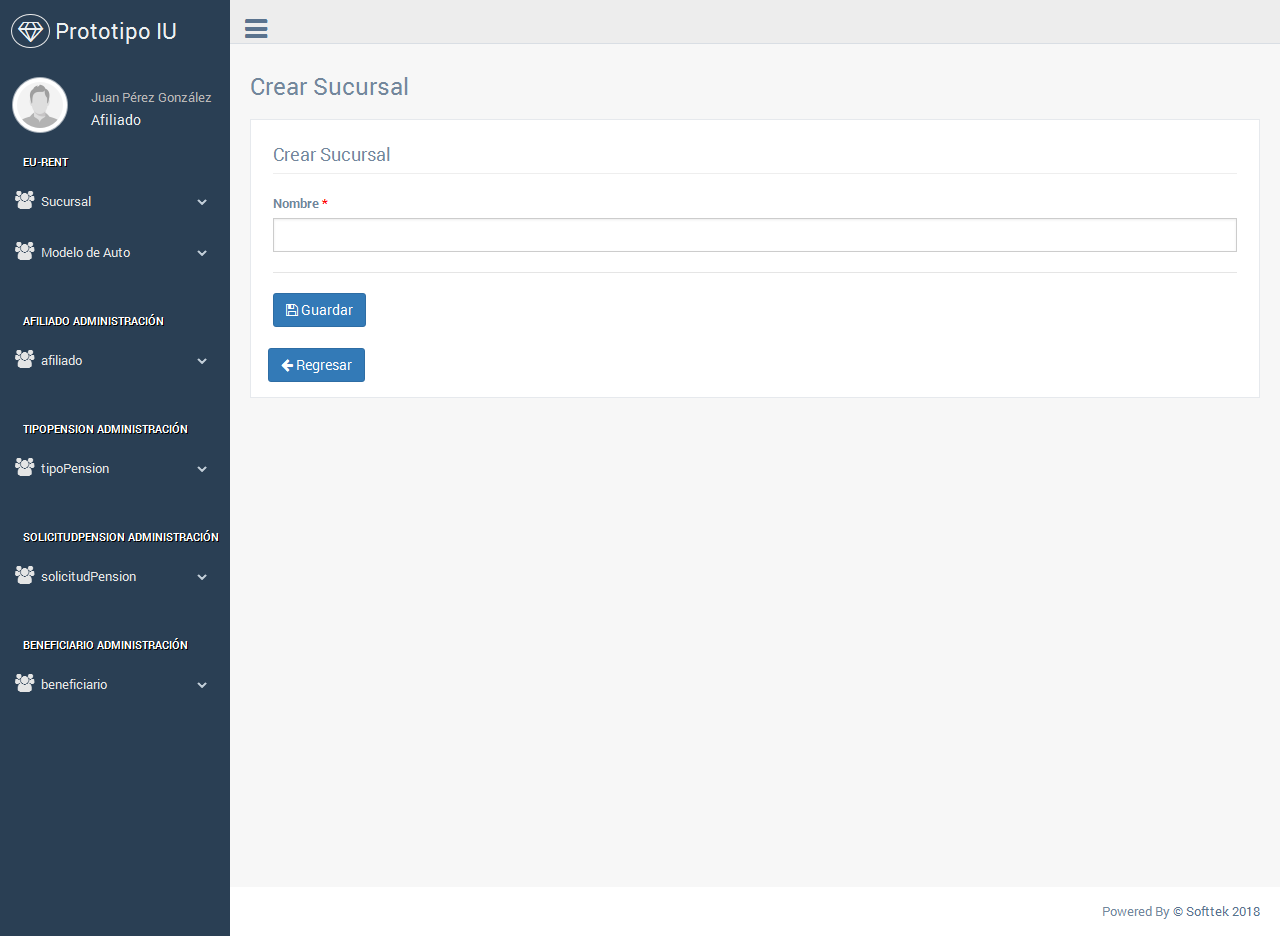
\includegraphics[width=\linewidth]{ui-prototype/SucursalServices/CrearSucursalPage.png}

\subsection{Buscar Modelo de Auto}

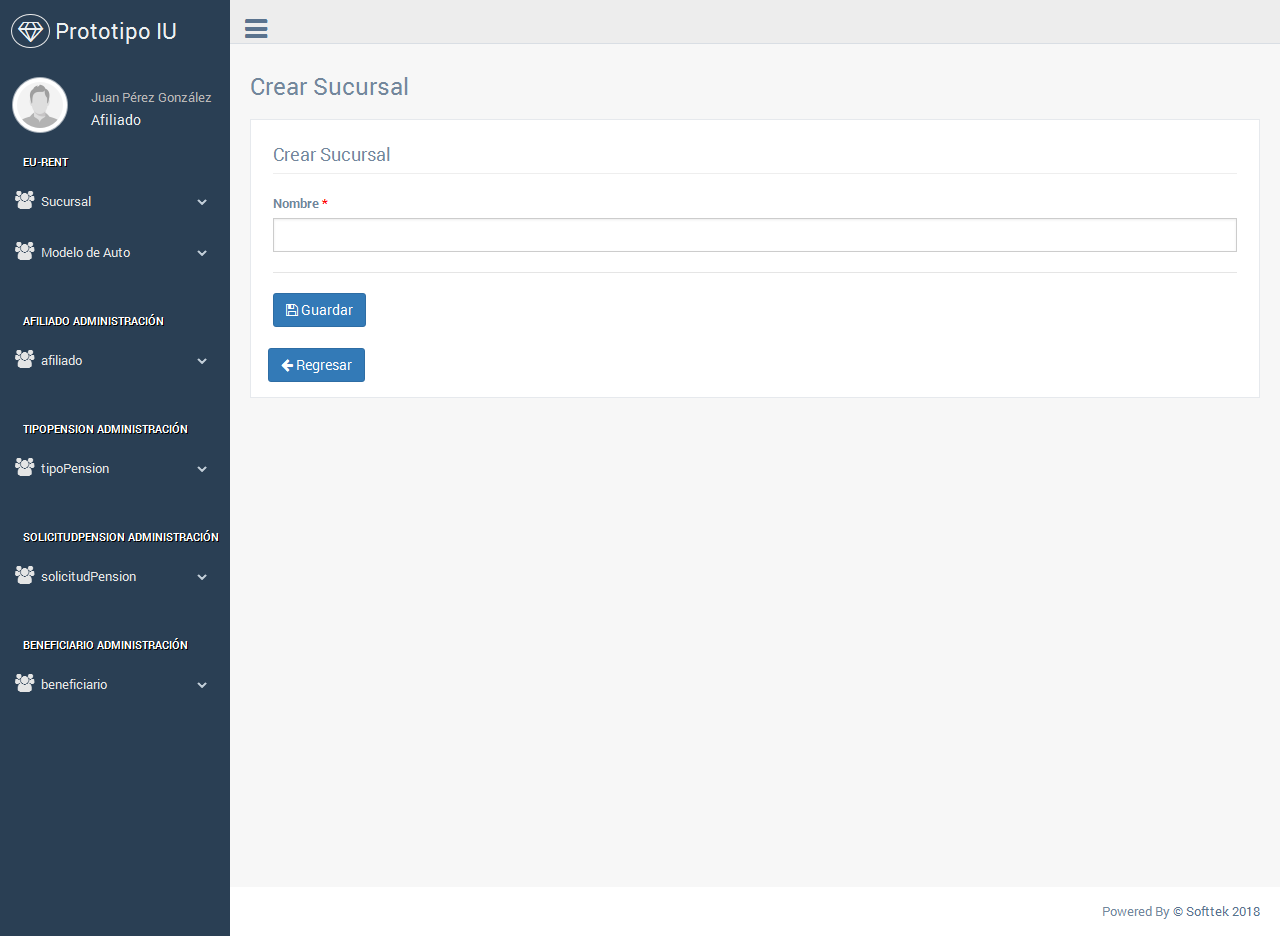
\includegraphics[width=\linewidth]{ui-prototype/SucursalServices/CrearSucursalPage.png}

\subsection{Editar Modelo de Auto}

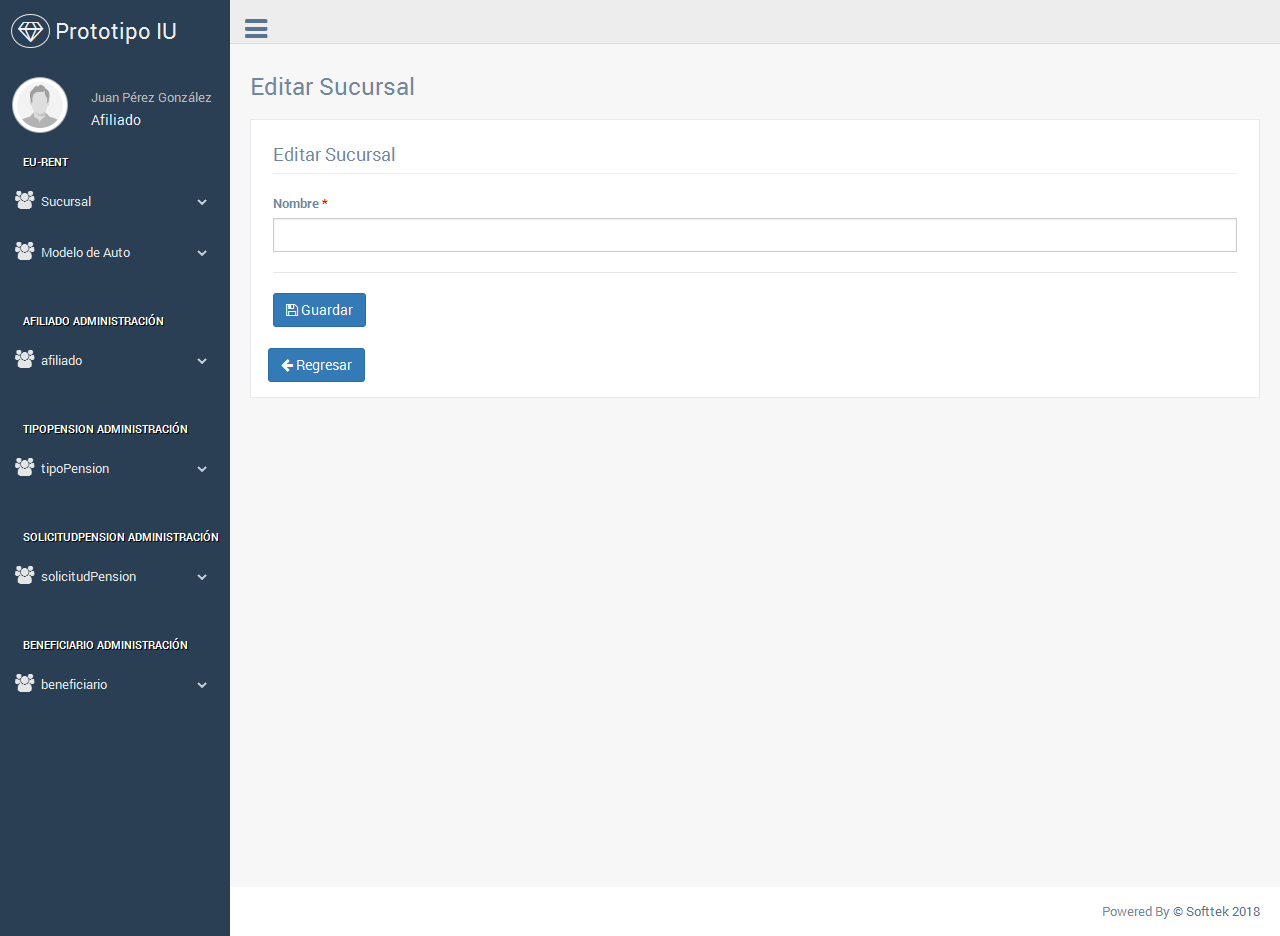
\includegraphics[width=\linewidth]{ui-prototype/SucursalServices/EditarSucursalPage.png}

\subsection{Eliminar Modelo de Auto}

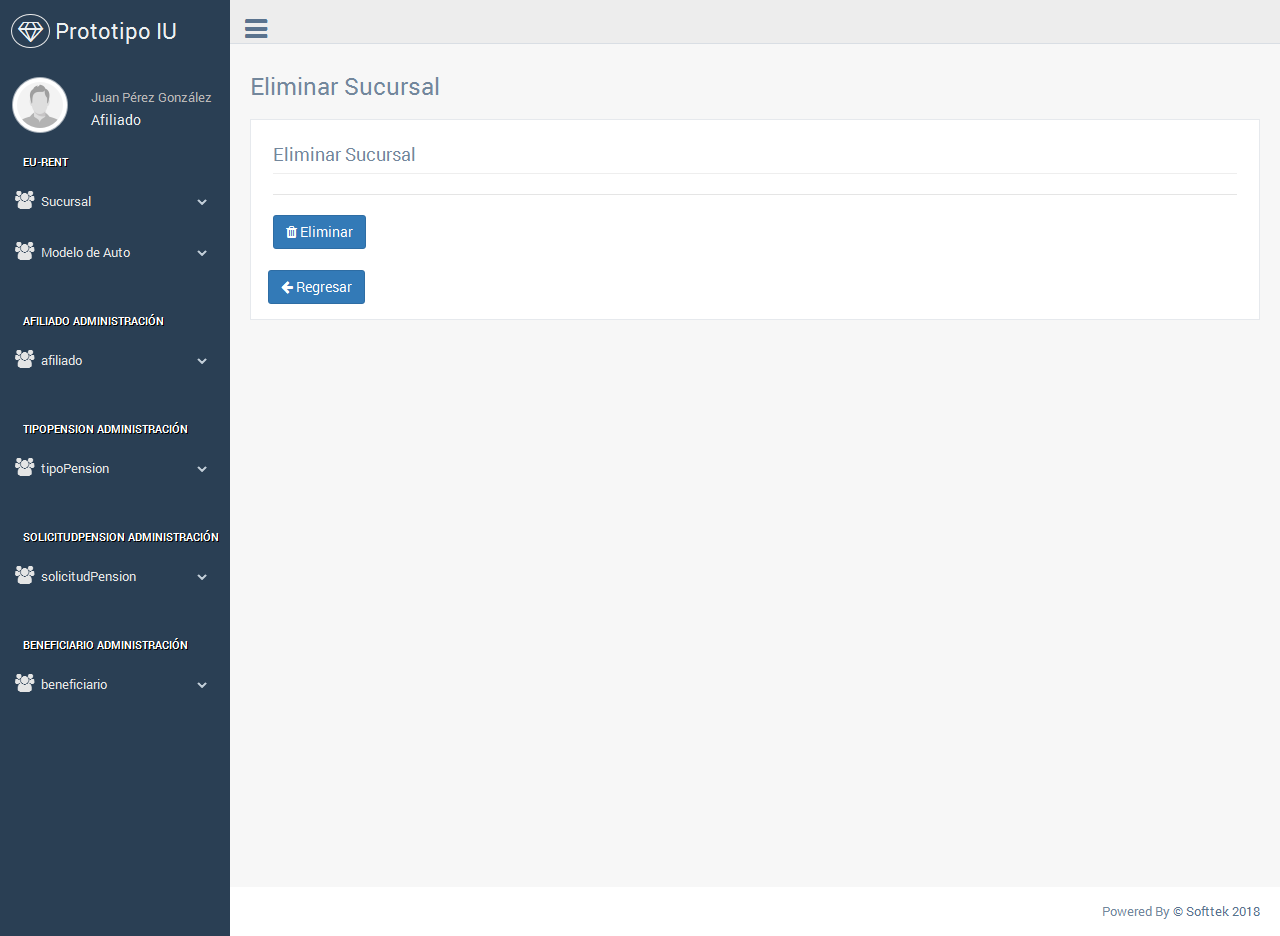
\includegraphics[width=\linewidth]{ui-prototype/SucursalServices/EliminarSucursalPage.png}

%\input{content/pantallas}

\clearpage

\printglossary

\end{document}